
\section{Kết quả kiểm thử từng thành phần}
\label{sec:component_testing}

Trước khi tiến hành phân tích hiệu năng, các thử nghiệm chức năng được thực hiện để xác nhận rằng từng thành phần của hệ thống hoạt động đúng như thiết kế.  
Các log tiêu biểu và hình ảnh minh họa dưới đây cho thấy quá trình khởi tạo, kết nối, truyền dữ liệu định kỳ, phát hiện té ngã, xử lý cảnh báo và truyền hình ảnh.

\subsection{Module cảm biến đeo}
Module Quectel EC800K thuộc phần cứng cảm biến đeo được kiểm tra để xác nhận khả năng giao tiếp AT command, thiết lập kết nối 4G và thu nhận dữ liệu GPS.  

Quy trình kiểm thử bao gồm: khởi tạo UART, kiểm tra thông tin modem và SIM, đánh giá chất lượng sóng, cấu hình APN, kích hoạt PDP context, bật GPS và truy vấn tọa độ, sau đó tắt GPS và ngắt kết nối dữ liệu để tiết kiệm năng lượng.  

Kết quả cho thấy module hoạt động ổn định: thiết bị nhận diện đúng (EC800K), SIM sẵn sàng, tín hiệu mạnh (\texttt{+CSQ: 31,99}), kết nối dữ liệu thành công và thu được tọa độ GPS hợp lệ.

\textbf{Log tiêu biểu:}
\begin{minted}[fontsize=\footnotesize,breaklines]{text}
I (2329) SIM_4G: Received: Quectel EG800K
OK
I (5329) SIM_4G: Received: +CSQ: 31,99
OK
I (28339) SIM_4G: Received: +QIACT: 1,1,1,"9.204.251.200"
OK
I (34349) SIM_4G: Received: +QGPSLOC: 10.88862,106.77975
OK
\end{minted}

\textit{Kết luận:} Module 4G/GPS đã hoạt động đúng chức năng, đảm bảo hệ thống có thể gửi cảnh báo và thông tin định vị qua SMS/MQTT.

\subsection{Khởi tạo hệ thống và kết nối mạng}
Quá trình khởi tạo xác nhận rằng các module SIM4G-GPS, Wi-Fi và các tác vụ chính đều hoạt động bình thường, đảm bảo thiết bị sẵn sàng tham gia vào quá trình truyền thông và giám sát.

\begin{minted}[fontsize=\footnotesize,breaklines]{text}
I (9961) SIM4G_AT: Initializing SIM4G AT driver...
I (9981) SIM4G_AT: Successfully set APN to v-internet
I (10011) APP_MAIN: System initialization complete.
I (10021) APP_MAIN: Application started successfully
\end{minted}

\textit{Kết luận:} Hệ thống đã khởi tạo thành công, chứng minh nền tảng phần mềm và phần cứng được tích hợp ổn định.

\subsection{Kết nối MQTT và truyền dữ liệu}
Thiết bị ESP32 kết nối thành công với broker MQTT và thực hiện gửi bản tin định kỳ chứa thông tin định danh, trạng thái té ngã và dữ liệu GPS.  

\begin{minted}[fontsize=\footnotesize,breaklines]{text}
I (19961) USER_MQTT: MQTT_EVENT_CONNECTED
I (39991) JSON_WRAPPER: Created status payload:
{"device_id":"ESP32_DEV_76E48B","fall_detected":false,
 "latitude":0,"longitude":0,"has_gps_fix":false}
\end{minted}

\begin{figure}[H]
    \centering
    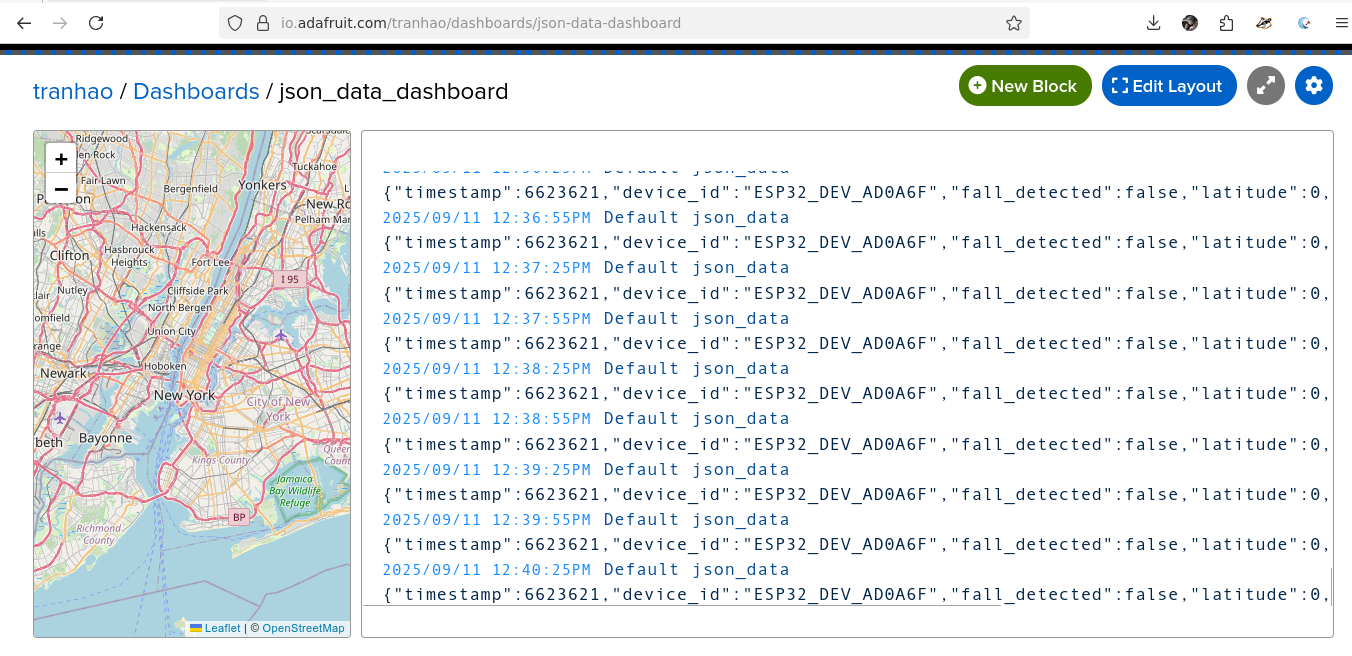
\includegraphics[width=0.8\textwidth]{figures/json_data_dashboard.png}
    \caption{Dashboard hiển thị bản tin MQTT từ thiết bị ESP32.}
    \label{fig:mqtt_dashboard}
\end{figure}

\textit{Kết luận:} Kết nối MQTT ổn định, đảm bảo thiết bị có thể truyền dữ liệu định kỳ tới hệ thống giám sát trung tâm.

\subsection{Phát hiện té ngã và xử lý cảnh báo}
Thuật toán phát hiện ghi nhận chuỗi trạng thái từ \texttt{LOW\_G} sang \texttt{HIGH\_G}, sau đó xác nhận va chạm và kích hoạt cảnh báo.  
Cảnh báo bao gồm gửi SMS, publish bản tin MQTT, đồng thời kích hoạt buzzer và LED cục bộ.  

\begin{minted}[fontsize=\footnotesize,breaklines]{text}
E (159131) FALL_LOGIC: FALL DETECTED! Accel: 0.99 g
I (159151) SIM4G_GPS: SMS request queued successfully
I (159191) SIM4G_GPS: MQTT alert published successfully.
I (159221) buzzer: Beeping for 8000 ms
I (159881) SIM4G_AT: SMS sent successfully.
I (175241) EVENT_HANDLER: Alert sequence completed.
\end{minted}

\begin{figure}[H]
    \centering
    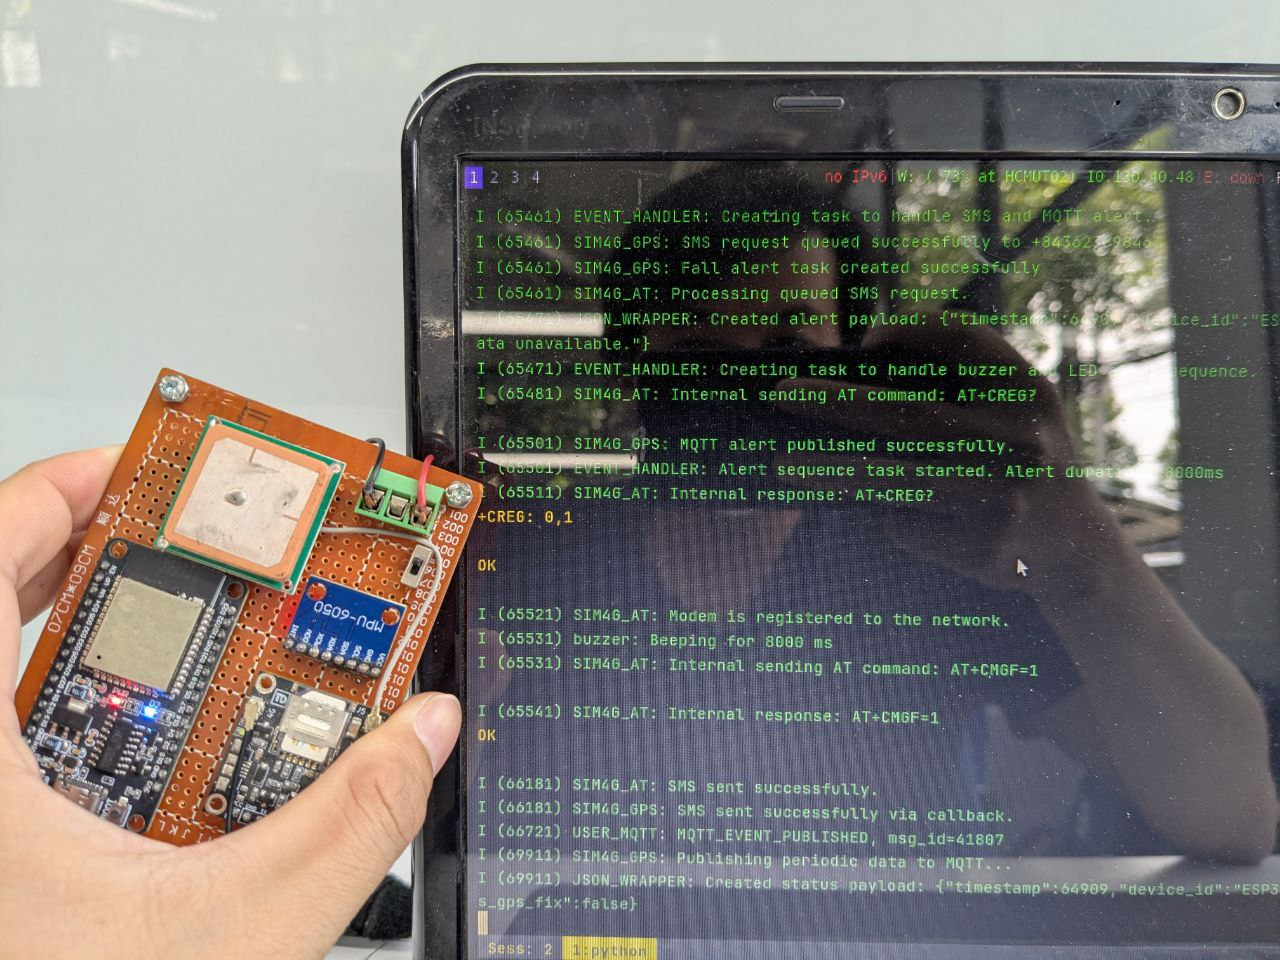
\includegraphics[width=0.8\textwidth]{figures/module1_real_log.jpg}
    \caption{Log thực tế của module cảm biến đeo khi phát hiện té ngã và kích hoạt cảnh báo.}
    \label{fig:module1_real_log}
\end{figure}

\textit{Kết luận:} Hệ thống phát hiện và xử lý cảnh báo té ngã thành công, kích hoạt đồng thời nhiều kênh cảnh báo.

\subsection{Module Camera và truyền hình ảnh}
Module ESP32-CAM được kiểm tra để xác nhận khả năng kết nối Wi-Fi và phát luồng hình ảnh qua HTTP.  
Kết quả log cho thấy camera được nhận diện đúng (OV5640), server HTTP đã khởi động và tốc độ khung hình trung bình dao động trong khoảng 3.5–5 FPS.
\begin{figure}[H]
    \centering
    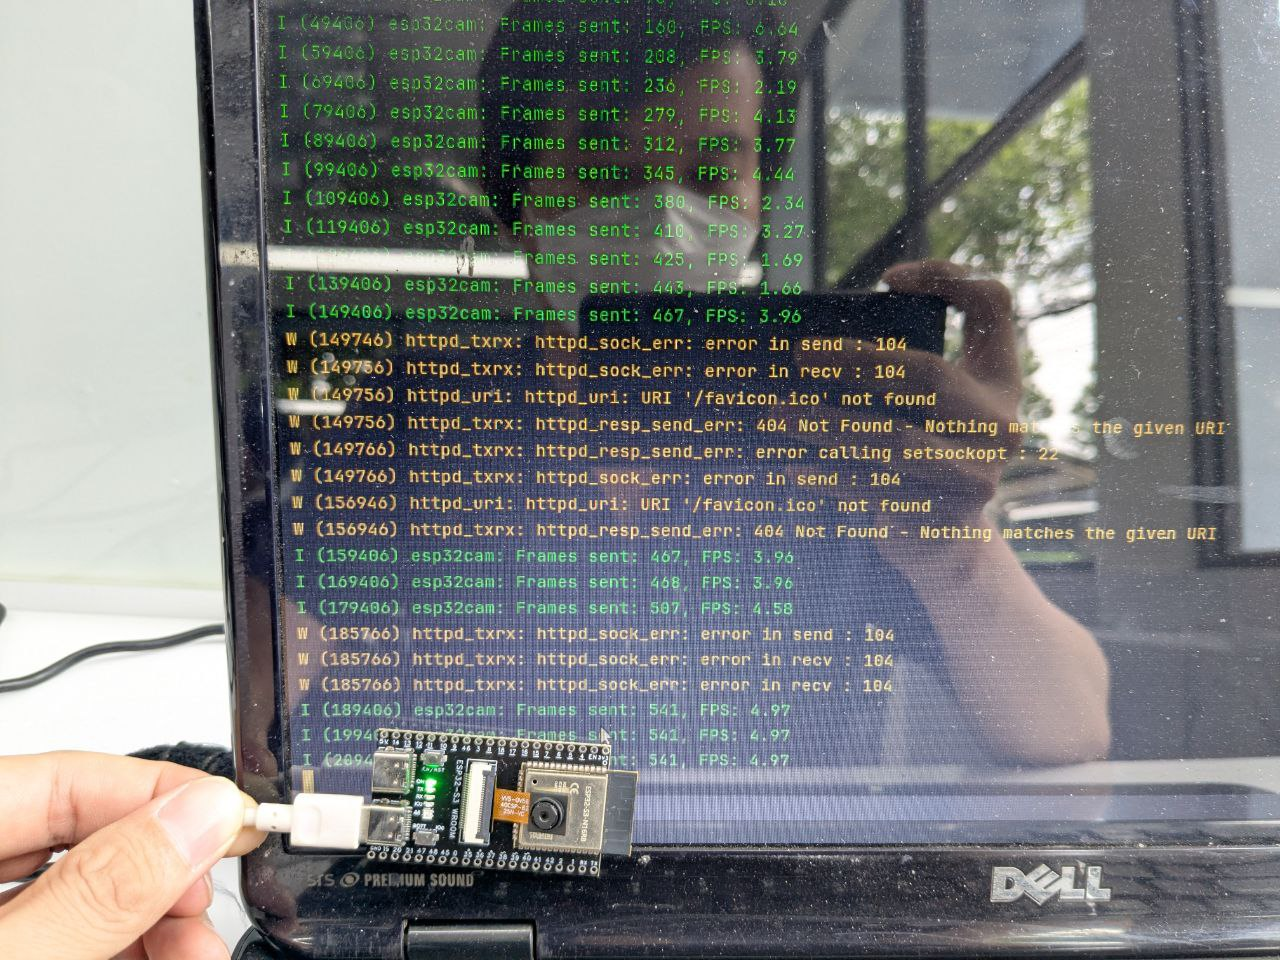
\includegraphics[width=0.8\textwidth]{figures/module2_real_log.jpg}
    \caption{Log thực tế của module esp-camera.}
    \label{fig:module2_real_log}
\end{figure}


\begin{minted}[fontsize=\footnotesize,breaklines]{text}
I (8936) esp32cam: Got IP: 10.110.87.85
I (9266) camera: Detected OV5640 camera
I (10006) esp32cam: HTTP server started
I (20006) esp32cam: Frames sent: 50, FPS: 5.87
I (40006) esp32cam: Frames sent: 146, FPS: 4.46
\end{minted}

\begin{figure}[H]
    \centering
    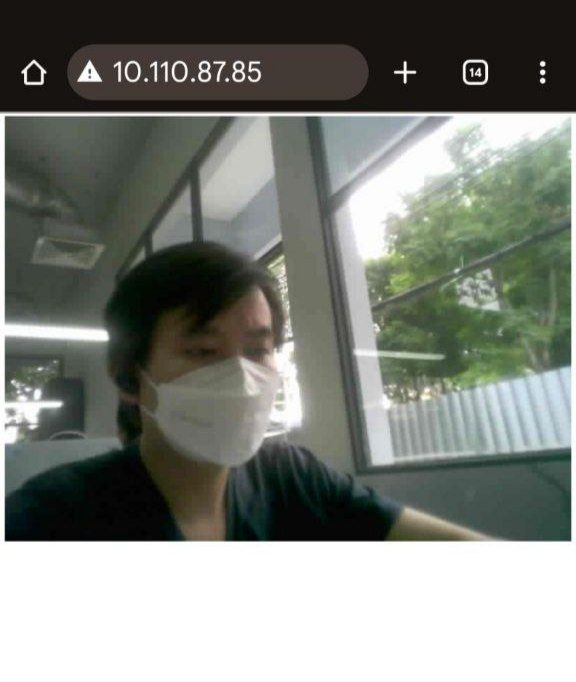
\includegraphics[width=0.8\textwidth]{figures/module2_stream_example.jpg}
    \caption{Luồng hình ảnh phát từ module ESP32-CAM qua HTTP.}
    \label{fig:camera_stream}
\end{figure}

\textit{Kết luận:} Module camera hoạt động ổn định, cho phép giám sát hình ảnh trực tiếp phục vụ xác minh sự kiện té ngã.

\subsection{Xử lý hình ảnh Python}
Module xử lý hình ảnh bằng Python nhận luồng video từ camera ESP32-CAM hoặc webcam, sau đó sử dụng TensorFlow Lite để phát hiện người và trích xuất các điểm khớp (skeleton) theo thời gian thực.  

Quy trình xử lý bao gồm:
\begin{itemize}
    \item Khởi tạo pipeline nhận luồng video từ camera.  
    \item Tiền xử lý khung hình (chuẩn hóa kích thước, màu sắc).  
    \item Chạy mô hình học máy TensorFlow Lite để phát hiện và trích xuất các điểm khớp của cơ thể người.  
    \item Vẽ skeleton trực quan trên khung hình để theo dõi trạng thái và chuyển động.  
\end{itemize}

Kết quả thực nghiệm cho thấy module hoạt động ổn định, xử lý khung hình theo thời gian thực với tốc độ trung bình 3--5 FPS.  
Hình~\ref{fig:python_skeleton} minh họa giao diện theo dõi người và skeleton được module xử lý hình ảnh tạo ra trong quá trình chạy thử nghiệm.

\begin{figure}[H]
    \centering
    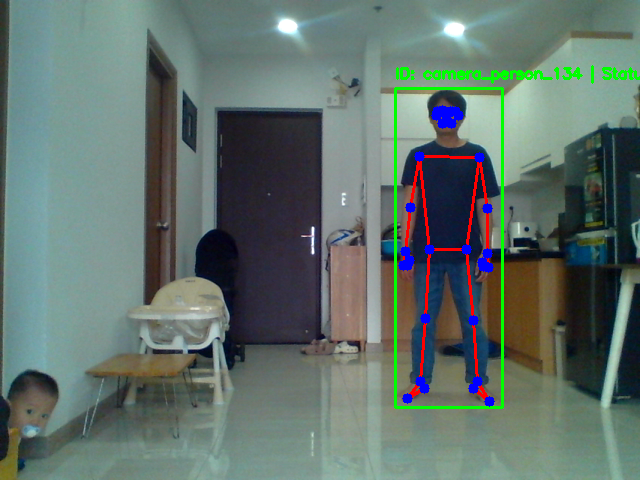
\includegraphics[width=0.85\textwidth]{figures/fall_detection_screen_shoot.png}
    \caption{Module Python xử lý hình ảnh: phát hiện người và vẽ skeleton theo thời gian thực.}
    \label{fig:python_skeleton}
\end{figure}

\subsection{Đánh giá thực nghiệm cảm biến mpu,gps và dữ liệu thu thập}
\subsubsection*{Quy trình thử nghiệm}
Để đánh giá hiệu quả hoạt động của hệ thống trong thực tế, quy trình thử nghiệm được tiến hành theo các bước:
\begin{enumerate}
    \item Nạp chương trình vào ESP32 bằng \texttt{idf.py flash monitor}.  
    \item Giả lập tình huống té ngã bằng cách lắc mạnh hoặc thả nhẹ thiết bị.  
    \item Quan sát log hệ thống để xác nhận sự kiện.  
    \item Kiểm tra tính năng gửi cảnh báo SMS với dữ liệu GPS.  
    \item Lặp lại nhiều lần để đánh giá tính ổn định và độ nhạy.
\end{enumerate}

\subsubsection*{Phân tích dữ liệu cảm biến}
Trong quá trình thử nghiệm, dữ liệu MPU6050 được thu thập cho hai trạng thái: \textbf{té ngã} và \textbf{bình thường}.  
Các bảng dưới đây trình bày dữ liệu đã ghi nhận.

\begin{table}[h]
\centering
\caption{Dữ liệu trong tình huống té ngã}
\label{tab:fall_data}
\begin{tabular}{|c|c|c|c|c|c|c|c|}
\hline
\textbf{Gyro X} & \textbf{Gyro Y} & \textbf{Gyro Z} & \textbf{Gyro Mag} & \textbf{Accel X} & \textbf{Accel Y} & \textbf{Accel Z} & \textbf{Accel Mag} \\
\hline
129.60 & -36.77 & 29.19 & 137.84 & 0.65 & 0.79 & -0.79 & 1.29 \\
-43.90 & 214.79 & 52.97 & 225.54 & 0.53 & 2.00 & -2.00 & 2.88 \\
158.75 & 250.13 & 134.18 & 325.22 & -1.18 & 1.72 & 1.56 & 2.61 \\
-250.14 & -246.07 & -250.14 & 430.91 & 1.11 & 2.00 & -2.00 & 3.04 \\
242.56 & 250.13 & 250.13 & 428.91 & -1.33 & -2.00 & 2.00 & 3.13 \\
-11.60 & -146.43 & -169.58 & 224.35 & 1.80 & 2.00 & -2.00 & 3.35 \\
201.32 & 238.97 & 250.13 & 400.25 & -2.00 & 0.21 & 2.00 & 2.84 \\
-250.14 & -250.14 & -250.14 & 433.25 & 0.55 & 0.23 & -0.37 & 0.69 \\
\hline
\end{tabular}
\end{table}

\begin{table}[h]
\centering
\caption{Dữ liệu trong tình huống bình thường}
\label{tab:normal_data}
\begin{tabular}{|c|c|c|c|c|c|c|c|}
\hline
\textbf{Gyro X} & \textbf{Gyro Y} & \textbf{Gyro Z} & \textbf{Gyro Mag} & \textbf{Accel X} & \textbf{Accel Y} & \textbf{Accel Z} & \textbf{Accel Mag} \\
\hline
1.27 & -1.46 & 0.51 & 2.00 & -0.03 & 0.01 & -0.96 & 0.96 \\
1.07 & -0.95 & 0.53 & 1.52 & -0.04 & 0.02 & -0.97 & 0.97 \\
1.18 & -1.36 & 0.73 & 1.94 & -0.03 & 0.02 & -0.97 & 0.97 \\
1.03 & -1.02 & 0.40 & 1.50 & -0.03 & 0.01 & -0.97 & 0.97 \\
1.37 & -1.08 & 0.58 & 1.84 & -0.03 & 0.01 & -0.97 & 0.97 \\
0.77 & -0.83 & 0.47 & 1.23 & -0.03 & 0.01 & -0.97 & 0.97 \\
1.02 & -0.37 & 0.77 & 1.33 & -0.03 & 0.01 & -0.97 & 0.97 \\
\hline
\end{tabular}
\end{table}

\begin{table}[h]
\centering
\caption{Bảng kết quả thu được từ log test của mô-đun 4G/GPS}
\label{tab:gps_data}
\begin{tabular}{|c|c|c|c|c|c|c|}
\hline
\textbf{Time (UTC)} & \textbf{Latitude} & \textbf{Longitude} & \textbf{Altitude (m)} & \textbf{Fix Mode} & \textbf{Date} & \textbf{Satellites} \\
\hline
132517.00 & 1053.3115N & 10646.7839E & 5.07 & 3 & 240425 & 07 \\
132517.00 & 1053.3115N & 10646.7839E & 5.07 & 3 & 240425 & 07 \\
132540.00 & 1053.3117N & 10646.7840E & 5.05 & 3 & 240425 & 07 \\
132540.00 & 1053.3117N & 10646.7840E & 5.05 & 3 & 240425 & 07 \\
132627.00 & 1053.3107N & 10646.7839E & 5.02 & 3 & 240425 & 07 \\
132627.00 & 1053.3107N & 10646.7839E & 5.02 & 3 & 240425 & 07 \\
\hline
\end{tabular}
\end{table}
% Bảng dữ liệu té ngã
% Bảng dữ liệu bình thường
% Bảng dữ liệu GPS
% Bảng so sánh

\textit{Kết luận:} Dữ liệu cảm biến cho thấy sự khác biệt rõ rệt giữa hai trạng thái. Đặc biệt, \textbf{Accel Mag} và \textbf{Gyro Mag} là chỉ báo hiệu quả để phát hiện té ngã, cung cấp cơ sở thực nghiệm cho việc tinh chỉnh ngưỡng phát hiện và giảm thiểu cảnh báo sai.


\subsection{Thử nghiệm Asterisk Call/SMS Gateway}
\label{sec:asterisk_test}

Trong hệ thống, Asterisk được sử dụng như một cổng trung gian để gửi cảnh báo bằng SMS và có tiềm năng mở rộng sang chức năng gọi điện tự động.  
Trong quá trình thử nghiệm, việc kích hoạt nhắn tin SMS qua Asterisk hoạt động thành công, cho phép hệ thống gửi cảnh báo đến số điện thoại đã đăng ký.  

Tuy nhiên, chức năng gọi thoại chưa được triển khai ổn định. Khi thay đổi máy chủ Asterisk, cấu hình giữ nguyên nhưng khả năng khởi tạo và duy trì cuộc gọi không đồng nhất. Điều này cho thấy còn tồn tại sự phụ thuộc vào môi trường triển khai, cần được nghiên cứu và tối ưu thêm trong tương lai.  

\begin{figure}[H]
    \centering
    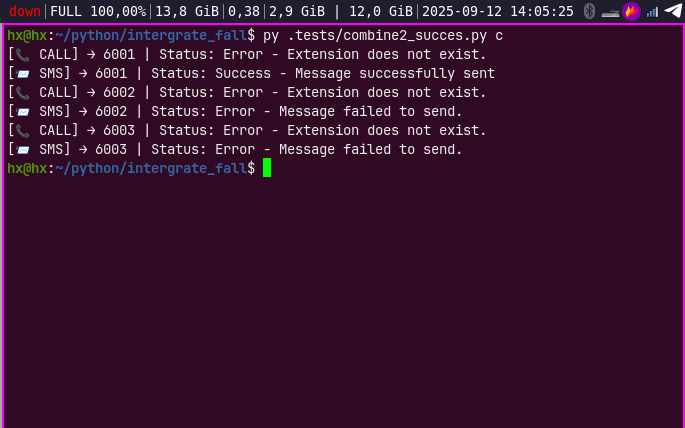
\includegraphics[width=0.8\textwidth]{figures/ast_call_sms_test.png}
    \caption{Thử nghiệm gửi SMS cảnh báo qua Asterisk.}
    \label{fig:ast_call_sms_test}
\end{figure}

\textit{Kết luận:} Module Asterisk đã hỗ trợ thành công chức năng nhắn tin SMS trong hệ thống. Chức năng gọi thoại vẫn còn hạn chế và sẽ cần nghiên cứu bổ sung để đảm bảo tính ổn định khi triển khai thực tế.

\subsection{Kênh cảnh báo Telegram}
\label{sec:telegram_alert}

Hệ thống Telegram Bot đóng vai trò là kênh cảnh báo trực quan, giúp gửi thông báo đến người dùng ngay khi phát hiện té ngã.  
Cơ chế hoạt động được chia thành hai hướng:
\begin{itemize}
    \item \textbf{Từ module phần cứng (ESP32 + 4G/GPS):} Khi xảy ra sự kiện té ngã, bản tin MQTT hoặc SMS được phát ra từ thiết bị. Hệ thống trung tâm sau đó chuyển tiếp nội dung này đến người dùng thông qua Telegram.
    \item \textbf{Từ module xử lý hình ảnh (Python):} Khi nhận diện được té ngã qua camera và skeleton, hệ thống Python trực tiếp gửi cảnh báo đến Telegram, kèm thông tin chi tiết.
\end{itemize}

\begin{figure}[H]
    \centering
    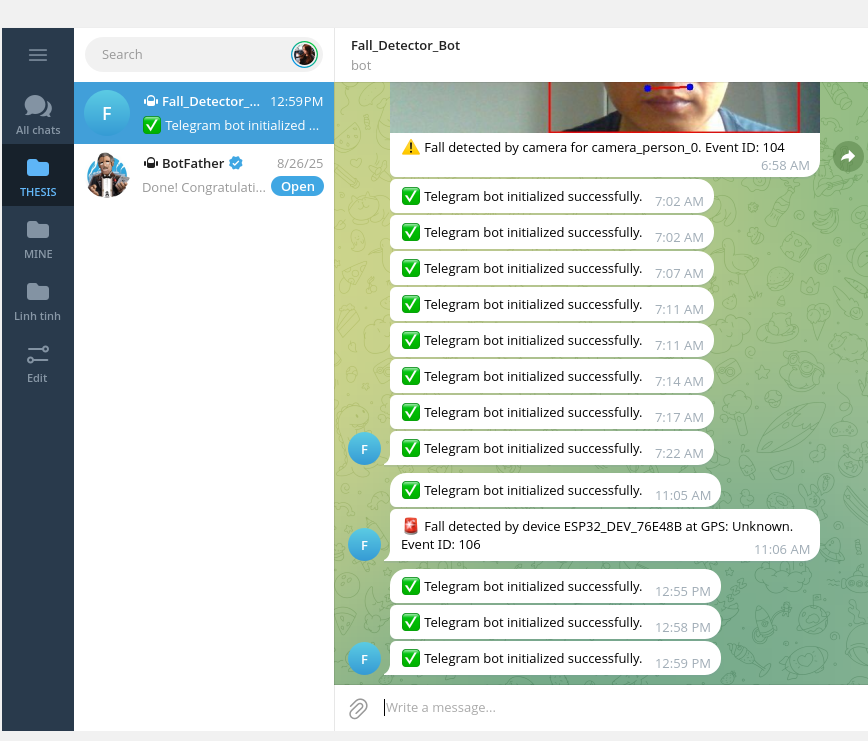
\includegraphics[width=0.8\textwidth]{figures/telegram_fall_module1_send.png}
    \caption{Thông báo cảnh báo té ngã từ module phần cứng (ESP32) qua Telegram.}
    \label{fig:telegram_hw}
\end{figure}

\begin{figure}[H]
    \centering
    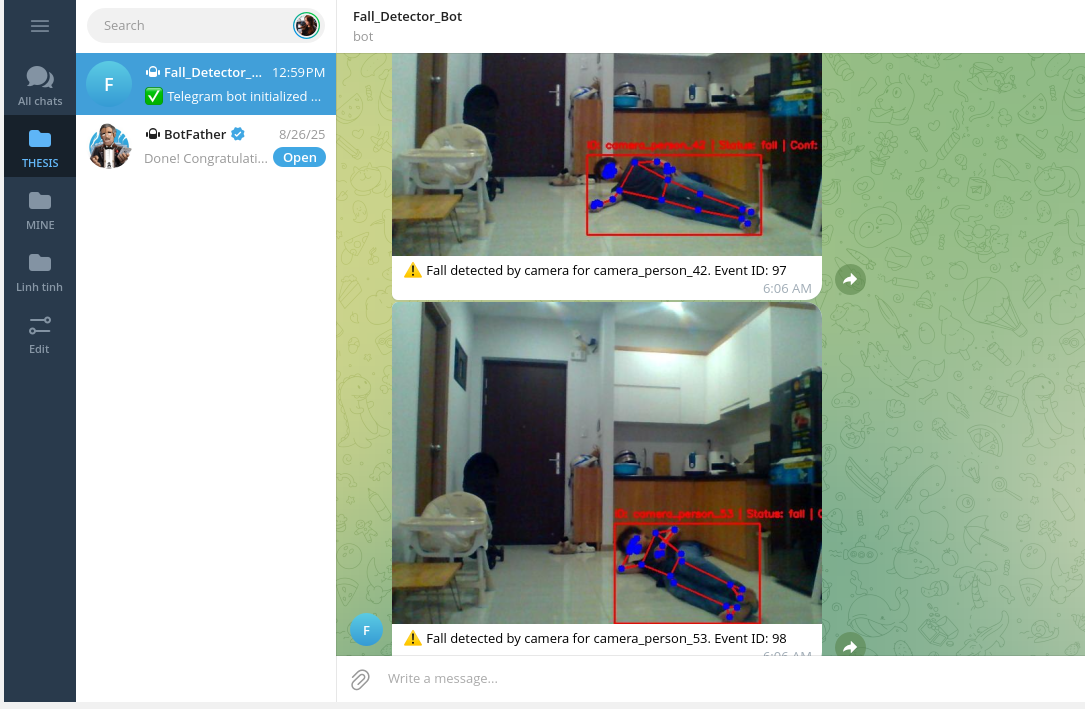
\includegraphics[width=0.8\textwidth]{figures/telegram_python_fall_send.png}
    \caption{Thông báo cảnh báo té ngã từ module xử lý hình ảnh Python qua Telegram.}
    \label{fig:telegram_python}
\end{figure}

\textit{Kết luận:} Kênh Telegram đã hoạt động ổn định, đóng vai trò cầu nối giữa hệ thống phát hiện té ngã và người dùng cuối. Việc kết hợp cả hai nguồn cảnh báo (thiết bị phần cứng và module xử lý hình ảnh) giúp tăng độ tin cậy và giảm thiểu khả năng bỏ sót sự kiện.
